\documentclass[a4paper,14pt]{extreport}

\usepackage{bsustyle/style/bsumain}
\usepackage{bsustyle/style/bsudiplomatitle}
\usepackage{blindtext}
\subfaculty{Кафедра вычислительной математики}


\title{УСКОРЕНИЕ СХОДИМОСТИ ПРОЦЕССОВ УСТАНОВЛЕНИЯ. ПЕРЕОБУСЛАВЛИВАНИЕ И ПОДАВЛЕНИЕ КОМПОНЕНТ}
\author{Касияник Алексей Леонидович}
\mentor{Фалейчик Борис Викторович \\
        кандидат физ.-мат. наук, \\
        доцент кафедры выч. мат.\\
        ~\\
        Бондарь Иван Васильевич \\
        магистр физ.-мат. наук, \\
        ассистент кафедры выч. мат.
        }
      
\reviewer{Зав. кафедры вычислительной математики\\
          кандидат физико-математических наук, доцент\\
          Мандрик Павел Алексеевич }

\begin{document}
  \maketitle
  
  \setcounter{page}{2}
\newpage
\chapter*{РЕФЕРАТ}

Дипломная работа, \pageref{LastPage}~страниц, \totfig~рисунков, 8 источников.
~\\

ПРИНЦИП УСТАНОВЛЕНИЯ, ЖЁСТКИЕ ЗАДАЧИ, МЕТОД РУНГЕ-КУТТЫ, СОБСТВЕННЫЕ ЗНАЧЕНИЯ, СПЕКТРАЛЬНЫЙ РАДИУС, ПЕРЕОБУСЛОВЛИВАНИЕ, ПОДАВЛЕНИЕ КОМПОНЕНТ, УСКОРЕНИЕ СХОДИМОСТИ
~\\

\textit{Объект исследования} – методы решения жёстких задач.
~\\

\textit{Цель работы} – разработка вычислительного алгоритма для решения жёстких дифференциальных задач на основе принципа установления.
~\\

\textit{Методы исследования} – методы численного анализа.
~\\

\textit{Результатом} является алгоритм решения жёстких дифференциальных задач с ускореной сходимостью, в основе которого лежит принцип установления.
~\\

\textit{Областью применения} является решение задач математической физики.

\chapter*{РЭФЕРАТ}

Дыпломная праца, \pageref{LastPage}~старонак, \totfig~малюнкаў, 8 крыніц.
~\\

ПРЫНЦЫП УСТАЛЯВАННЯ, ЖОРСТКІЯ ЗАДАЧЫ, МЕТАД РУНГЕ-КУТТЫ, УЛАСНЫЯ ЗНАЧЭННІ, СПЕКТРАЛЬНЫ РАДЫУС, ПЕРААБУМОЎЛЕННЕ, ПАДАЎЛЕННЕ КАМПАНЕНТ, ПАСКАРЭННЕ ЗБЕЖНАСЦІ
~\\

\textit{Аб'ект даследавання} – метады рашэння жорсткіх задач.
~\\

\textit{Мэта працы} – распрацоўка вылічальнага алгарытму для рашэння жорсткіх задач на аснове прынцыпа ўсталявання.
~\\

\textit{Метады даследавання} – метады лічбавага аналізу.
~\\

\textit{Вынікам} з'яўляецца алгарытм рашэння жорсткіх дыферэнцыяльных задач з паскоранай збежнасцю, у аснове якога ляжыць прынцып усталявання.
~\\

\textit{Вобласцю выкарыстання} з'яўляецца рашэнне задач матэматычнай фізікі.

\chapter*{Abstract}
Bachelor's thesis, 42 pages, 20 figures, 34 sources.
~\\

STEADYING PRINCIPLE, STIFF PROBLEMS,  RUNGE-KUTTA METHODS, EIGENVALUES, SPECTRAL RADIUS, PRECONDITIONING, COMPONETS OPRESSION,  CONVERGENCE ACCELERATION.
~\\

\textit{Object of research} -- methods for solving stiff problems.
~\\

\textit{The purpose of the work} -- development of computational algorithm for solving stiff differential problems on the basis of the steadying principle.
~\\

\textit{Research methods} -- methods of numerical analysis.
~\\

\textit{The result} is an algorithm for solving stiff differential problems with the acceleration of convergence, which is based on the steadying principle.
~\\

\textit{The field of application} is the solution of problems of mathematical physics.

  {
    \renewcommand{\contentsname}{Содержание}
    \tableofcontents
  }

  \chapter*{Введение}
  \addcontentsline{toc}{chapter}{Введение}
  Жесткие задачи исследуются примерно со второй половины 20 века. Однако и сейчас сформулировать точное определение жесткости проблематично. Наиболее прагматическая точка зрения вместе с тем была и исторически наиболее ранней (Кертисс и Хиршфельдер, 1952 год): \textit{жесткие уравнения — это уравнения, для которых определенные неявные методы дают лучший результат, обычно несравненно более хороший, чем явные методы.} При этом определенную роль играют собственные значения матрицы Якоби, но важны и такие параметры, как размерность системы, гладкость решения или интервал интегрирования. 
Более полным является определение данное Ламбертом: \textit{если численный метод с ограниченной областью абсолютной устойчивости, примененный к системе с произвольными начальными условиями вынужден использовать на некотором интервале интегрирования величину шага, которая чрезмерно мала по отношению к гладкости точного решения на этом интервале, тогда говорят, что система является жесткой на этом интервале}\cite{hairer}.


Как известно, наиболее трудоёмким этапом численного интегрирования жёсткой системы (не)линейных обыкновенных дифференциальных уравнений (ОДУ) размерности $n$ неявным методом является решение на каждом шаге системы (не)линейных уравнений, размерность которой пропорциональна n. В таком случае использование методов ньютоновского типа практически невозможно, а традиционные методы типа простой итерации либо не сходятся, либо сходятся очень медленно. В данной работе рассматриваются способы ускорения методов, основанных на процессах установления, которые применимы в указаной выше ситуации.
В работе исследованы два эффективных способа ускорения сходимости методов установления: переобусловливание и подавление компонент.Переобусловливание  является классическим способом улучшения обусловленности задачи, что существенным образом определяет свойства сходимости.

Также в процесе решения у нас появляется некоторая дополнительная информация о свойствах решаемой задачи. Эта информация может быть также использована для ускорения сходимости. В результате исследования данного феномена был предложен прием ускорения итерационного процесса, который  по аналогу со схожими алгоритмами из известных источников именуется «подавлением компонент».
Исследованию описанных проблем, разработке вычислительного алгоритмов, которые бы основывались на идее установления и при этом превосходили в скорости известные алгоритмы и посвящается данная работа.
  \label{c:intro}


  \chapter{Жесткие задачи}
  \label{c:stiff_problems}
  Тема численного решения однородных дифференциальных уравнений не нова, и, возможно, несколько удивителен тот факт, что методы, разработанные еще в начале 20 века, до сих пор являются основой наиболее эффективных и распространенных подходов при решении ОДУ. За прошедшее время были достигнуты значительные продвижения в надежности и эффективности этих методов, и большинство существующих типичных научных задач могут быть решены достаточно легко и быстро. Тем не менее есть некоторый класс задач, с которыми классические методы справиться не могут. Такие задачи, называемые «жесткими», слишком важны, чтобы их игнорировать, и слишком трудны, чтобы их решить. Они слишком важны, чтобы их игнорировать, так как они возникают при решении важных физических задач. Они слишком затратные при решении, так как из-за присущей им большой размерности и сложности, классические методы становятся слабо применимы даже несмотря на многократное увеличение мощности современной вычислительной техники. Классические методы решения требуют так много шагов, что ошибки округления могут сделать полученное решение далеким от приемлемого[2]. В этом разделе мы и рассмотрим понятие «жесткости», а также те ключевые проблемы, которые возникают при их решении.

  \section{Явление жесткости}
  \label{s:stiffness}
  Задачи, называемые жесткими, весьма разнообразны, и дать математически строгое определение жесткости непросто. Поэтому в литературе можно встретить различные определения жесткости, отличающиеся степенью строгости. Сущность же явления жесткости состоит в том, что решение, которое необходимо вычислить, меняется медленно, однако в любой его окрестности существуют быстро затухающие возмущения. Характерное время затухания их называют пограничным слоем. Наличие таких возмущений затрудняет получение медленно меняющегося решения численным способом. При этом жесткими могут быть как скалярные дифференциальные уравнения, так и, что встречается особенно часто, системы обыкновенных дифференциальных уравнений.
  
  
\begin{Definition}Система обыкновенных дифференциальных уравнений вида
  \begin{equation}
  \label{stiff:eq}
    u'(t)=Au(t)
  \end{equation}
  с постоянной $(n \times n)$-матрицей $ A $ называется жесткой, если: 
  \begin{enumerate}
  \item $Re\lambda _k <0, k=\overbar{1,n}$ (т.е. задача устойчива);
  \item Отношение $S = \dfrac{\max\limits_{1\leq k\leq n} |Re\lambda _k|}{\min\limits_{1\leq k\leq n} |Re\lambda _k|} $ велико (например, $S > 10$);
  \item Промежуток интегрирования велик по сравнению с длиной погранслоя.[Repn]
  \end{enumerate}
\end{Definition}

Число $S$ иногда называют \textit{коэффициентом жесткости} системы. 


Поскольку система нелинейных обыкновенных дифференциальных уравнений вида $u'(t)=f(t, u(t))$ может быть в окрестности некоторого известного решения $v(t)$ заменена линейной системой 
$$u'(t) = f_u (t, v + \theta (u-v))u + b(t), $$
где $f_u$ - матрица Якоби, а $b(t) = f(t, v)-f_u(t,v + \theta (u-v))v$, то понятие жесткости для нелинейных систем может быть определено аналогично. Заметим, однако, что за пределами класса систем линейных обыкновенных дифференциальных уравнений с постоянной матрицей полагаться на спектр как на источник надежной информации о распространении погрешности уже нельзя[Dekker, Verver].

  
  \section{Трудности, возникающие при численном решении}
  \label{s:stiff_troubles} Трудность численного решения жестких систем обыкновенных дифференциальных уравнений выражается в нескольких аспектах. При использовании традиционных явных пошаговых методов, основы которых были заложены более века назад, возникают сильные ограничения на длину шага интегрирования.
  
  
  Рассмотрим в качестве примера систему из двух независимых уравнений   
  \begin{equation}
  \label{stiff:system}
  \begin{cases}
   u_1'(t)=-\lambda_1 u_1(t), 
   \\
    u_2'(t)=-\lambda_2 u_2(t), t>0, \lambda_2 \gg \lambda_1 > 0.
  \end{cases}
  \end{equation}
  Эта система имеет решение $u(t)=(u_1(t), u_2(t))^T = (u_1^0 e^{-\lambda_1 t}, u_2^0 e^{-\lambda_2 t})^T$. При выписанных условия на $\lambda_1$ и $\lambda_2$, очевидно, компонента $u_2(t)$ решения затухает гораздо быстрее, чем $u_1(t)$ и, начиная с некоторого момента $t$ поведение вектора $u(t)$ почти полностью определяется компонентой $u_1(t)$. Однако при решении системы \eqref{stiff:system} численным методом величина шага интегрирования, как правило, определяется компонентой $u_2(t)$, не существенной с точки зрения поведения решения системы. Например, используя явный метод Эйлера, мы из первого уравнения имеем ограничения на шаг $\tau \le 2/\lambda_1$, а из второго - $\tau \le 2/\lambda_2$ и, таким образом, ясно, что для решения системы \eqref{stiff:system} как цельного математического объекта шаг $\tau$ ограничен величиной $2/\lambda_2$. Такая же ситуация типична и при решении любой системы обыкновенных дифференциальных уравнений вида \eqref{stiff:eq}.
  
Учитывая выше сказанное, можно сделать вывод, что для решения жестких задач наиболее пригодны те численные методы, которые требуют наиболее слабых ограничений на величину шага численного интегрирования из соображений устойчивости. Таким образом, традиционные явные пошаговые методы, основы которых были заложены более века назад, мало пригодны из-за сильных ограничений на длину шага интегрирования, обусловленных неудовлетворительными свойствами устойчивости таких методов. 

 
 Начиная с пятидесятых годов двадцатого столетия, для интегрирования жестких задач стали применяться неявные одно- и многошаговые методы, обладающие хорошими свойствами устойчивости. Они позволяют находить приближенное решение жестких задач на достаточно больших шагах. Наиболее эффективными на данный момент считаются неявные коллокационные методы типа Рунге–Кутты. Однако и эти методы обладают существенным недостатком, который состоит в необходимости решения на каждом шаге системы нелинейных уравнений, размерность которой пропорциональна размерности дифференциального уравнения и количеству стадий метода. Поэтому машинная реализация таких методов является весьма громоздкой, и, кроме того, возникающие системы нелинейных уравнений в общем случае могут быть неразрешимы. Применение неявных методов также затрудняется необходимостью вычисления матрицы Якоби.
 
 
 Стоит затронуть еще один важный момент, не относящийся напрямую к проблеме жесткости. Это вопрос о контроле точности приближенного решения. При пошаговом интегрировании для этих целей обычно используется техника «откатов»: если вычисленная (по правилу Рунге, например) оценка погрешности недостаточно мала, полученное приближение отбрасывается и вычисления повторяются заново с уже меньшей длиной шага. Такой подход, во-первых, не экономичен, так как полностью игнорируется полученное на данном шаге приближенное решение, которое может быть достаточно близким к точному. Вместо того, чтобы уменьшать шаг и повторять такие же вычисления, можно попытаться каким-то образом уточнить уже имеющееся приближение. Во-вторых, несколько «откатов» подряд могут привести к недопустимо малым
значениям шага \cite{Faleichik_Vych_alg}.

В настоящее время наиболее часто для этих целей используют либо неявные методы, либо методы, специально сконструированные для решения задач конкретного вида[Repnikov]. Хорошо применимыми при решении жестких систем являются методы, основанные на процессах установления, которые и рассматриваются в главе~\ref{c:stead_methods}. 

  
  \section{Примеры жестких задач}
  \label{s:stiff_examples}  
  Обширные численные эксперименты с жесткими задачами впервые провели Энрайт, Халл и Линдберг (1975). Их набор задач STIFFDETEST является стандартом для проверки качественности численных методов решения жестких систем \cite{hairer}. В данном разделе приводятся некоторые тестовые задачи, которые в дальнейшем будут использованы в численном эксперименте.
  
  \subsection{HIRES: Модель дифференциации растительной ткани}
  \label{ss:hires}
  HIRES -- это химическая реакция с участием восьми реагентов была предложена Шефером (1975) для объяснения "роста и дифференциации растительной ткани независимо от фотосинтеза при высоких уровнях светового облучения". Готтвальд (1977) предложил использовать ее в качестве тестового примера\cite{hairer}.
  
 Данный пример -- типичный случай биохимической модели «умеренной» размерности (современные модели, например, фотосинтеза включают сотни уравнений подобного типа). Хотя данная модель является умеренно жесткой, тем не менее, ее лучше решать с помощью методов, предназначенных для решения жестких систем ОДУ\cite{holodov}.
   
   Соответствующие уравнения имеют вид:
    \begin{equation}
	\begin{aligned}
	\label{hires}
	&y_1' = -1.71 y_1+0.43 y_2+8.32 y_3+0.0007,\\
	&y_2' = 1.71y_1 - 8.75y_2,\\
	&y_3' = -10.03y_3+0.43y_4+0.035y_5,\\
	&y_4' = 8.32y_2 + 1.71y_3-1.12y_4,\\
	&y_5' = -1.745y_5 + 0.43y_6 + 0.43y_7,\\
	&y_6' = -280y_6y_8+0.69y_4+1.71y_5-0.43y_6+0.69y_7,\\
	&y_8'=-y7';\\
	&\\
	y_1(0)&=1, y_2(0) = y_3(0) = ...=y_7(0) = 0, y_8(0) = 0.0057,
	\end{aligned}
	\end{equation}
и для выдачи были выбраны значения $x_{out}=312.8122$ и $421.8122$.

\subsection{ROBER: Модель химических реакций Робертсона}
  \label{ss:rober}
  Один из первых и самых популярных примеров жесткой системы ОДУ принадлежит Робертсону (1966) и имеет вид, типичный для моделей химической кинетики -- в правой части системы стоят полиномы второй степени от концентраций.
  
  ROBER -- реакция Робертсона имеет вид:
   \begin{equation}
	\begin{aligned}
	\label{rober}
	&y_1' = -0.04y_1+10^4 y_2y_3,\\
	&y_1' = 0.04y_1-10^4y_2y_3 -3 \cdot 10^7y_2^2,\\
	&y_3' = 3\cdot10^7y_2^2;\\
	\\
	y_1&(0)=1, y_2(0) = 0, y_3(0) = 0.
	\end{aligned}
	\end{equation}
Обычно эту задачу рассматривали на отрезке $0 \leq x \leq 40$, пока Хайндмарш не обнаружил, что многие программы терпят неудачу, если $x$ становится очень большим (например, $10^11$). Причина заключается в том, что как только компонента численного решения $y_2$ случайно становится отрицательной, онап стремится к $-\infty$, и выполнение программы прекращается из-за переполнения. Поэтому для выдачи выбирают значения:
$$ x_{out}=1, 10, 10^2, 10^3, ..., 10^{11}$$


\subsection{OREGO: Модель Филда–Нойса «орегонатор»}
  \label{ss:orego}
OREGO -- орегонатор, знаменитая модель с периодическим решением, описывающая реакцию Белоусова-Жаботинского:
\begin{equation}
	\begin{aligned}
	\label{orego}
	&y_1' = 77.27(y_2+y_1(1-8.375\cdot10^{-6}y_1-y_2)),\\
	&y_1' = \dfrac{1}{77.27}(y_3-(1+y_1)y_2),\\
	&y_3' = 0.161(y_1-y_3),\\
	\\
	y_1&(0)=1, y_2(0) = 2, y_3(0) = 3, & x_{out}=30, 60, 90, ..., 360.
	\end{aligned}
	\end{equation}
	На то, что система жесткая, указывают большие различия в константах скоростей реакций -- есть процессы «быстрые», и есть «медленные».
Так как переменные системы — концентрации ($HBrO_2$, $Br^{-}$ и $Ce(IV)$ соответственно), то начальные условия для системы  выбирают положительными и, как правило, достаточно близкими к $0$.


\subsection{Одномерное уравнение теплопроводности}
  \label{ss:teploprov}
  
  
  

  \chapter{Методы установления}
  \label{c:stead_methods}
  В настоящей главе приводятся основные сведения о вычислительном алгоритме, основанном на идее установления. Рассмотриваются случаи применения как к линейной системе, так и к нелинейной системе обыкновенных дифференциальных уравнений. Линейный случай является исследуемым в численном эксперименте в главе~\ref{c:numer_ex}.
  
  \section{Линейная задача}
  \label{s:linear_problem}
Рассмотрим задачу Коши для неоднородной линейной системы обыкновенных дифференциальных уравнений (ОДУ):
	\begin{equation}
	\begin{aligned}
	\label{main_problem}
	&y'(t)=Jy(t)+f(t),\\
	&y(t_0)=y_0,\\
	&t \in [t_0, t_0+\tau],\quad \\
	&y_0\in \mathbb{R}^N,\quad
	y:[t_0,t_0+\tau] \to \mathbb{R}^N,\quad\\
	&J \in \mathbb{R}^N \times \mathbb{R}^N, \quad
	\tau \in [0, +\infty).\\
	\end{aligned}
	\end{equation} 
Для нахождения приближения к $y(t_0 + \tau), \tau > 0$ проинтегрируем её произвольным s-стадийным неявным методом типа Рунге-Кутты. Далее этот метод будем называть \textit{базовым методом}. Базовый метод может быть представлен следующей таблицей Бутчера:
	\begin{center}
	\begin{equation}
	\label{base_method}
	\begin{array}{l|lll}
	c_1& a_{11}& ...& a_{1s}\\
	...& ...& ...& ...\\
	c_s& a_{s1}& ...& a_{ss}\\
	\hline
	& b_1& ...& b_s\\
	\end{array}
	\end{equation}
	\end{center}
Здесь $A=(a_{i,j})_{i,j=1}^s$ - так называемая матрица Бутчера
базового метода. Тогда
	$$ y(t_0+\tau)\thickapprox y_1=y_0+\tau\sum_{i=1}^sb_ik_i,$$
где $\{k_i\}_{i=1}^s$ находятся как решение следующей системы линейных алгебраических уравнений (СЛАУ)
	$$k_i = J(y_0+\tau\sum_{j=1}^sa_{ij}k_j)+f(t_0+c_i\tau).$$
В дальнейшем будем пользоваться матричной записью этой СЛАУ:
	\begin{equation}\label{system_for_solving}
	\begin{aligned}
	&(\tau A\otimes J-I)k+g=0,\\
	&g=(g_1,g_2,..,g_s)^T, \quad g_i=f(t_0+c_i \tau)+Jy_0, \quad i=1,..,s,\\
	&k=(k_1,k_2,..,k_s)^T, \quad k_i \in \mathbb{R}^N.\\
	\end{aligned}
	\end{equation}
Здесь $\otimes$ обозначает кронекеровское произведение матриц[], по
определению которого получаем, что $$G=\tau A\otimes J-I$$ - блочная
матрица вида
	\begin{equation}
	\left(
	\begin{array}{llll}
	-1+\tau a_{11}J& \tau a_{12}J&...&\tau a_{1s}J\\
 	\tau a_{12}J&-1+\tau a_{22}J&...&\tau a_{2s}J\\
	...&...&...&...\\
	\tau a_{s1}J& \tau a_{s2}J&...&-1+\tau a_{ss}J\\
	\end{array}
	\right ).
	\end{equation}
	
Как правило, к \eqref{system_for_solving} применяются различные методы решения СЛАУ, как точные методы (LU-разложение), так и методы крыловского типа (проекционные методы). Однако, первые требуют значительных вычислительных затрат, а другие могут не давать удовлетворительной скорости сходимости. В этой же работе рассматривается альтернативный подход, основанный на процессах установления\cite{Bondar_Faleichik_Parall}.
	
 
Рассмотрим вспомогательное уравнение
	\begin{equation}
	\label{estEquation}
	k'=(\tau A\otimes J-I)k+g=Gk+g = r(k),
	\end{equation}
которое в дальнейшем будем называть уравнением установления.

Очевидно, что точное решение уравнения \eqref{system_for_solving} $k^*$ будет являться стационарным решением \eqref{estEquation}. Для этого достаточно, чтобы спектр матрицы $G$ целиком содержался в левой комплексной полуплоскости. Поэтому, если проинтегрировать~\eqref{estEquation}  каким-нибудь численным методом, то можно получить приближение к решению \eqref{system_for_solving}.

Для решения \eqref{estEquation} будем использовать явный метод Рунге-Кутты, задаваемый таблицей вида
	\begin{equation}
	\label{auxilary_method_table}
	\begin{array}{lllll}
	 \alpha_{21}& & & &  \\
	 \alpha_{31}&\alpha_{32} & & &  \\
	 ...& ...& ...& &\\
	 \alpha_{\sigma1}& \alpha_{\sigma2}&... &\alpha_{\sigma\sigma-1}&  \\
	\hline
	 \beta_1&\beta_2 &...&\beta_{\sigma-1}& \beta_\sigma\\
	\end{array}
	\end{equation}
В результате применения явного метода Рунге-Кутты, получаем семейство методов, именуемых итерационными процессами установления или обобщенными итерациями Пикара. 
	
Пусть $\omega$ - шаг по фиктивному времени. 
	\begin{equation}\label{ipe_gf}
	\begin{aligned}
	&k^{l+1}=\Phi(k^{l})\\
	&\Phi(k)=k+\omega \sum_{p=1}^\sigma\beta_pK_p(k),\\
	&K_p(k)=G (k +\omega\sum_{q=1}^{p-1}\alpha_{pq} K_q(k))+g.
	\end{aligned}
	\end{equation}
		
Учитывая специфику интегрирования уравнения установления \eqref{estEquation}, нужно выбрать  $\omega$, $\{\alpha_{ij}\}_{i,j=1}^{\sigma}$, $\{\beta_i\}_{i=1}^{\sigma}$. Один из способов выбора коэффициентов предложен в \cite{Faleichik_Bondar_Kyiv}. В частности, используя тот факт, что процесс \eqref{ipe_gf} может быть записан в виде 
	\begin{equation}
	\label{ipe_spektr}
	k^{l+1} = R_\sigma(\omega G)k^l+P(\omega, G),
	\end{equation}
	где $R_\sigma$ -- полином степени $\sigma$,  многочлен степени $\sigma$, называемый функцией устойчивости вспомогательного метода, $P$ -- некоторый многочлен от матрицы.
	
	Многочлен $R_\sigma$ определяет свойства устойчивости итерационного метода. В нашем случае, он определяет свойства сходимости итерационного процесса, а именно, область устойчивости
	$$ S = \{z \in \mathbb{C}\ :\  |R_{\sigma}(z)|<1  \}$$
должна содержать в себе  спектр матрицы $\omega G$ \cite{Faleichik_Bondar_Kyiv}.


Запишем многочлен устойчивости в виде
 $$R_{\sigma}(z)=1+\sum_{j=1}^\sigma a_jz^j,$$
где $z \in \mathbb{C}$. Коэффициенты $\{a_i\}_{i=1}^\sigma$, $a_i\in \mathbb{R}$ будем выбирать таким образом, чтобы минимизировать функцию
%$$u'(h)=\lambda u(h) +\varphi(h), \quad u(t_0) = u_0$$
%Выбор метода интегрирования~(\ref{estEquation}) будем производить следующим образом: построим множитель (многочлен) перехода таким образом, чтобы его область устойчивости как можно лучше покрывала  (обозначим её $\Omega(\alpha)$, $\Omega(\alpha)=\{(\rho,\varphi):|R(\rho e^{\mathrm i\varphi})|<1\}$ )
\begin{equation}
\label{minimizeR}
F(a_1,...,a_\sigma)=\int_0^1\int_{\pi-\alpha}^{\pi+\alpha}|R_\sigma(\rho e^{\mathrm i\varphi})|^2d\varphi
d\rho\
\end{equation}
Здесь $\alpha$ - некоторый заранее заданный угол, определяющий область устойчивости полинома $R_\sigma$ \cite{Faleichik_article},\cite{Faleichik_bondar_amade}. Вообще, $\alpha$ нужно выбирать исходя из представлений о спектре матрицы $G$, поскольку чем лучше будет приближен спектр, тем более эффективным будет метод. Параметр $\omega$ выбирается так, чтобы спектр матрицы $\omega G$ полностью содержался в области устойчивости. Для этого достаточно положить $\omega$ равным спектральному радиусу матрицы $G$.

Имея сконструированный многочлен устойчивости, мы можем восстановить матрицу Бутчера вспомогательного метода, используя подход, описанный в \cite{hairer}, \cite{Faleichik_amade}. Более подробно выбор коэффициентов вспомогательного метода описан в \cite{Bondar}.
  
  \section{Нелинейная задача}
  \label{s:non_linear_problem} 
  
Рассуждения для нелинейного случая проходят во многом аналогично случаю линейному, поэтому остановимся только на различиях.

Рассмотрим систему нелинейных дифференциальных уравнений
	\begin{equation}
	\begin{aligned}
	\label{nolin_main_problem}
	&y'(t)=f(t, y(t)),\\
	&y(t_0)=y_0,\\
	&t \in [t_0, t_0+\tau],\quad \tau>0 \\
	&y_0\in \mathbb{R}^N,\quad
	y:[t_0,t_0+\tau] \to \mathbb{R}^N,\quad\\
	&f:  \mathbb{R}^N \to \mathbb{R}^N.
	\end{aligned}
	\end{equation}
Для интегрирования воспользуемся методом \eqref{base_method}, причем в отличие от линейного случая применение запишем в симметричном виде:
	$$Y_i = y_0+\tau \sum_{j = 1}^s a_{i,j}f(t_0+c_j \tau,Y_j), $$
	$$y(t_0+\tau)\thickapprox y_1 = y_0 + \tau \sum_{j = 1}^s b_{j}f(t_0+c_i \tau,Y_j),$$
что в векторной форме представимо как
	\begin{equation}
	\begin{aligned}
	\label{nolin_system_for_solving1}
	&Y = e\otimes y_0 +\tau (A\otimes I)F(t_0,Y),\\
	&y_1 = e\otimes y_0 +\tau(b^T\otimes I)F(t_0,Y).
	\end{aligned}
	\end{equation}
Здесь $e = (1,..., 1)$, $e \in \mathbb R^s$,  $Y = (Y_1, ...,Y_s)^T$, $F(t, Y) =\\= \left(f(t+c_1 \tau,Y_1),..., f(t+c_s \tau,Y_s) \right)^T$.
Уравнение установления для \eqref{nolin_system_for_solving1} имеет вид
	\begin{equation}
	\label{nolin_estEquation} Y(\theta)'=\tau (A\otimes I)F(t_0,Y(\theta)) -Y(\theta)+ e\otimes y_0 = \tilde r(Y(\theta)).
	\end{equation}
Соответствующий ему процесс установления имеет вид аналогичный \eqref{ipe_gf}:
	\begin{equation}
	\label{nolin_ipe_gf}
	\begin{aligned}
	&Y^{l+1}=\Phi(Y^{l}),\\
	&\Phi(Y)=Y+\omega \sum_{p=1}^{\sigma}\beta_{p}K_p(Y),\\
	&K_p(Y)=\tilde r(t_0,Y+\omega \sum_{q=1}^{p-1}\alpha_{pq}K_q(Y)).
	\end{aligned}
	\end{equation}
Полностью повторить конструирование вспомогательного метода как в случае
линейной системы вообще говоря нельзя. Однако если задача позволяет, то можно
провести линеаризацию и исследовать спектральные свойства уже для неё, полностью
повторяя приведенные в [Bondar] рассуждения о конструировании вспомогательных методов.
Параметр $\omega$ полагаем таким, чтобы все собственные значения матрицы Якоби
правой части уравнения \eqref{nolin_estEquation} были по модулю меньше 1.
  
  \section{Спектральные свойства и скорость сходимости итерационного процесса}
  \label{s:spectral_speed} 
Как уже было сказано, процесс \eqref{nolin_ipe_gf} представим в следующем виде:
	\begin{equation}
	\label{ipe_spektr_form}
	k^{l+1} = R_\sigma(\omega G)k^l+P(\omega, G),
	\end{equation}
где $R_\sigma$ -- многочлен перехода (функция устойчивости),  $P$ -- функция, точный вид которой несущественен в данном случае.
	
	Мы уже определились, что многочлен перехода определяет свойства сходимости итерационного процесса, и положив $\omega$ равным спектральному радиусу матрицы $G$, получили, что спектр матрицы $\omega G$ будет полностью содержаться в области устойчивости. Таким образом, спектр матрицы $\omega G$ имеет определяющее влияние на сходимость итерационного процесса \eqref{nolin_ipe_gf}.

Предположим, что нам известен спектр исходной матрицы $J$, и отследим каким может быть спектр результирующей матрицы
	$$G = \tau(A\otimes J) - I.$$
По свойству кронекеровскго произведения матриц [Dekker], собственные значения $\nu_{i,j}$ матрицы $G$ равны
	\begin{equation}\label{spektrG}
	\nu_{ij} = \tau \mu_j \lambda_i - 1,
	\end{equation}
где $\mu_i$ -- собственные значения матрицы $A$, $\lambda_j$ - собственные значения матрицы $J$. То есть, над  спектром исходной матрицы системы \eqref{main_problem} производятся операции масштабирования,поворота и параллельного переноса. Собственные значения матрицы $\omega G$, очевидно, являются смасштабированными на единичный круг собственными значениями  $G$. 

Описанные преобразования могут привести к выходу спектра матрицы $G$ за пределы левой комплексной полуплоскости, что по определению плохо – процессы установления становится неприменимыми. Но даже если выход не произошел, нет гарантии что такая ситуация не возникнет при увеличении шага интегрирования по
времени. Чтобы избежать описанного выше нежелательного явления, можно осуществить так называемую операцию переобусловливания. Применение операции переобусловливания к методам установления подробно рассматривается  в главе~\ref{s:precond}.

Проследим как будет изменяться ошибка на $l$-ой итерации:$\varepsilon^l= k^* - k^l$. Учитывая \eqref{ipe_spektr_form}, получим:
	$$\varepsilon^l = R_\sigma (\omega G)\varepsilon^{l-1}$$
Далее предположим, что у матрицы $G$ имеется полный набор собственных векторов $\{\eta^i\}_{i=1}^N$. Тогда

	$$ \varepsilon^l = \sum_{i = 1}^{N}\varepsilon_i^{l-1}R(\omega G) \eta^i = 		\sum_{i=1}^{N}\varepsilon_i^{l-1}R(\omega \nu_i )\eta^i,$$
здесь $\nu_i$ -- собственное значение, соответствующее $\eta^i$. Таким образом,% получили соотношение для ошибки на $l$-ой итерации:
	$$ \varepsilon_i^l = R_\sigma(\omega \nu_i) \varepsilon_i^{l-1} = (R(\omega \nu_i))^l\varepsilon_i^0.$$
Проанализируем последнее выражение. $R_\sigma$ -- многочлен перехода, и по построению $R_\sigma(0) = 1$. Учитывая непрерывность $R_\sigma$, получим что $R_\sigma$ близок к 1 когда $\omega \nu_i$ близко к 0. Это значит, что компоненты ошибки, соответствующие малым величинам $\omega \nu_i$, будут уменьшаться медленно. Нетрудно видеть, что характеристикой,  в достаточной мере описывающей свойства сходимости, является так называемое ``спектральное число обусловленности'' матрицы $J$ исходной системы, $\varkappa = \rho(J) \rho(J^{-1})$ ($\rho$ здесь - спектральный радиус). Чем больше эта величина, тем медленнее будет сходиться итерационный процесс.
  
  \section{Переобусловливание}
  \label{s:precond}
  Решение системы линейных алгебраических уравнений вида
  \begin{equation}
	\label{slau}
	Ax=b,
	\end{equation}
 где $A$ -- $(n \times n)$-матрица коэффициентов, является центральной задачей многих численных моделей, и часто решение такой системы является наиболее трудоемкой частью вычислений. В вычислительной математике для ускорения сходимости итерационных методов решения таких систем часто применяют подход, известный как \textit{переобусловливание}. 
	
	Как известно, переобусловливание -- это процесс преобразования системы \eqref{slau}  в систему с улучшенными свойствами сходимости итерационного процесса. Вообще говоря, целью переобусловливания является уменьшение числа обусловленности матрицы: чем меньше число обусловленности матрицы, тем быстрее сходится итерационный процесс \cite{benzi}.
	
	Один из частных приемов такого подхода	заключается в решении умноженой слева исходной системы СЛАУ на некоторую невырожденную матрицу:
	\begin{equation}
	\label{precondslau1}
	MAx=Mb,
	\end{equation}
причем такой прием имеет смысл только в том случае, если число обусловленности матрицы коэффициентов $MA$ меньше, чем у исходной матрицы.	
	
	Матрица $M$, с помощью которой осуществляется такое преобразование, называется \textit{переобусловливателем}. 
  
  Решатели с переобуславливанием обычно эффективнее, чем использование простых решателей в случае больших и особенно в случае разреженных матриц. Итерационные решатели с переобуславливанием могут использовать безматричные методы, в которых матрица коэффициентов A не хранится отдельно, а доступ к ее элементам происходит через произведения матриц-векторов\cite{wiki-precond}.
  
  Переобусловленную слева систему также можно записать в виде 
  \begin{equation}
	\label{precondslau2}
	M(Ax-b)=0.
	\end{equation}
 Вообще говоря, хороший переобусловливатель $M$ должен удовлетворять следующим требованиям:	
 \begin{itemize}
 \item Переобусловленная система должна легко решаться.
 \item Переобусловливатель должен легко вычисляем и применим\cite{benzi}.
 \end{itemize}
 Первое свойство означает, что итерационный процесс должен быстро сходиться, в то же время, второе свойство говорит о том, что каждая итерация не должна быть слишком затратна. Заметим, то эти два тербования находятся в конкуренции между собой, и необходимо всегда соблюдать некий баланс между ними.
 
 Так наиболее легко вычисляемым переобусловливателем будет являться $M = I$. Очевидно, что применяя такой переобусловливатель, мы получим исходную СЛАУ, и смысла в таком переобусловливателе нет. Другая крайность, выбор в качестве переобусловливателя обратной матрицы исходной матрицы коэффициентов, т.е. $M = A^{-1}$. В этом случае итерационный процесс будет наиболее быстро сходится, т.к. будет получено оптимальное число обусловленности 1, требующее одной итерайции, чтобы процесс сошелся. Однако, поскольку нахождение обратной матрицы -- задача не тривиальная и более трудоемкая, чем решение исходной системы, построение переобуславлевателя такого вида на практике не целесообразно.  
	
	Как можно заметить, построение эффективного переобусловливателя может быть совсем не тривиальной задачей. Способы построения переобуславливателей в контексте процессов установления и приводятся в данной главе.
    
  \subsection{Первый способ}
  \label{ss:precond_1}
  Чтобы  избежать описанного в главе~\ref{s:spectral_speed} нежелательного явления, можно осуществить операцию переобусловливания \cite{gomel},\cite{konf_may}  умножив систему \eqref{system_for_solving} слева на $A^{-1}\otimes I$ (здесь $I\in \mathbb{R}^N \times \mathbb{R}^N $). Тогда система \eqref{system_for_solving} примет вид:
\begin{gather}\label{precond_system_for_solving}
%\begin{aligned}
(\tau I_s\otimes J-A^{-1}\otimes I_N)k+\tilde g=0,\\
\notag \tilde g=(\tilde g_1,\tilde g_2,..,\tilde g_s)^T, \quad \tilde g_i=(A^{-1}\otimes I_N)(f(t_0+c_i \tau)+Jy_0), \quad i=1,..,s,\\
\notag k=(k_1,k_2,..,k_s)^T, \quad k_i \in \mathbb{R}^N,
%\end{aligned}
\end{gather}
здесь $I_s$ и $I_N$ -- единичные матрицы размерности $s\times s$ и
$N \times N$ соответственно. Также стоит отметить, что точные
решения \eqref{system_for_solving} и
\eqref{precond_system_for_solving} совпадают. По свойствам
кронекеровского произведения, собственные значения
матрицы
$$\tilde G =(\tau I_s\otimes J-A^{-1}\otimes I_N) $$
равны
$$\tilde \nu_{ij} = \tau \lambda_i - \frac{1}{ \mu_j}.$$
Здесь отсутствует преобразование вращения, выполняются только
масштабирование и параллельный перенос.  Если все $\mu_j$ имеют
положительные вещественные части (а это справедливо для большинства
применяемых на практике методов Рунге--Кутты), то полностью
отсутствует опасность выхода спектра матрицы $\tilde G$ за пределы
левой комплексной полуплоскости. 

Кроме вышеописанной пользы, операция переобуславливания также позволяет сократить объем вычислений, а также позволяет экономить память при хранении $\tilde G$ в виде разреженной матрицы\cite{Bondar}.
  
  \subsection{Второй способ}
  \label{ss:precond_2}
  Еще один подход  к переобусловливанию связан с приближением обратной матрицы. Для этого используем особый тип переобуславливателей, известный как полиномиальный переобуславливатель $M=p_k(A)$ \cite{chen}:
	 \begin{equation}
	\label{polinom_precond1}
	p_k(A)Ax=p_k(A)b,
	\end{equation}
или
	 \begin{equation}
	\label{polinom_precond2}
	p_k(A)(Ax- b)=0,
	\end{equation}
где $p_k(A)$ -- многочлен от матрицы $k$-ой степени следующего вида:
	 \begin{equation}
	\label{polinom_precond3}
	p_k(A)=c_kA^k + c_{k-1}A^{k-1} + ... + c_1A+c_0.
	\end{equation}
Уже упоминалось, что наилучшим в смысле скорости сходимости итерационного процесса переобусловливателем является обратная матрица коэффициентов системы алгебраических уравнений. Вместо точного вычисления обратной матрицы, что, очевидно,  не целесообразно, попробуем найти какое-то ее приближение, используя приведенный выше полиномиальный переобусловливатель \eqref{polinom_precond3}, т.е. попытаемся найти приближение обратной функции от матрицы.

 Как известно, для того, чтобы определить какую-либо функцию от матрицы, достаточно определить ее на спектре матрицы. Предположим, что у нас имется некоторая квадратная матрица $A$ размерности $N$  c полным набором собственных значений ${\lambda_i}^N_{i=1}$. Также для простоты изложения предполагаем, что собственные значения все различны и среди них нету нулевых значений. Тогда произвольную функцию  от матрицы $A$ можно записать в виде:
	 \begin{equation}
	\label{invf1}
	f(A)=\sum_{i=1}^{N} f(\lambda_i) \prod_{j  \neq i} \dfrac{A - \lambda_j}{\lambda_i - \lambda_j}
	\end{equation}
В частности, для обратной функции
	$$
	f_{inv}(x) = x^{-1} 
	$$
имеем 
	 \begin{equation}
	\label{invf2}
	f_{inv}(A) =\sum_{i=1}^{N} f(\lambda_i^{-1}) \prod_{j  \neq i} \dfrac{A - \lambda_j}{\lambda_i - \lambda_j}.
	\end{equation}
Если нам известны все собственные значения матрицы коэффициентов $A$, то переобуславливатель
	 \begin{equation}
	\label{invf3}
	M =f_{inv}(A)
	\end{equation}
будет в точности равен обратной матрице для матрицы $A$. Отметим, что,  как правило, спектр матрицы $A$ неизвестен, но можно оценить границы, в которых находятся собственные значения. Предположим, нам известны числа $a, b$, такие, что
	$$
	a \leq \lambda_1 \leq \lambda_2 \leq ... \leq \lambda_N \leq b,
	$$
где $\lambda_1, ..., \lambda_N$ -- упорядоченные по возрастанию собственные значения матрицы $A$. Тогда можно приблизать функцию $f_{inv}(x)$ на отрезке $[a, b]$ каким либо способом. Например, проинтерполировав многочленом Лагранжа по чебышовским узлам на этом отрезке.  Пусть $q$ -- степень интерполяционного многочлена. Узлы ${p_i}_{i=0}^q$, распределенные на отрезке $[a, b]$ вычисляются по известным формулам:
 	\begin{equation}
	\label{precondLagr1}
	p_i = \dfrac{b+a}{2} +\dfrac{b-a}{2}\cos(\dfrac{\pi(2i+1)}{2q+2}), i=\overbar{1, q}
	\end{equation}
В качестве переобусловливателя тогда будетвыступать многочлен
	\begin{equation}
	\label{precondLagr2}
	p_q(A) =\sum_{i=1}^{N} f(p_i^{-1}) \prod_{j  \neq i} \dfrac{A - p_j}{p_i - p_j}.
	\end{equation}.

В численом эксперименте в качестве переобусловливателя будем использовать наименее уклоняющийся от обратной функции $\dfrac{1}{1-t}$ на промежутке $(\dfrac{-1}{\gamma}, \dfrac{1}{\gamma})$ полином $f(t)$. Очевидно, что 
$$f(t) = \gamma F(\gamma t),$$
где $F(t)$ есть полином, наименее уклоняющийся от функции $\dfrac{1}{\gamma - t}$ на промежутке $(-1, 1)$. Подход ускорения итерационных процессов, основанный на использовании функции $f(t)$ , в литературе известен как универсальный алгоритм, наилучший в смысле второго критерия\cite{fadeev}.

Полином степени $s-1$, удовлетворяющий последнему требованию, был известен еще Чебышеву. Именно, 
	\begin{equation}
	\label{chebyshev1}
	F_{s-1}(t) =-\dfrac{2\alpha^{\frac{s}{2}}}{(1-\alpha)^2} \dfrac{1}{\gamma - t}\left[T_s(t) - 2\sqrt{\alpha} T_{s-1}(t) + \alpha T_{s-2}(t)\right] + \dfrac{1}{\gamma - t},
	\end{equation} 
где 
	$$
	\alpha= (\gamma - \sqrt{\gamma^2 - 1})^2, T_s(t) = \cos s \arccos t.
	$$

Таким образом,  
	\begin{equation}
	\label{chebyshev2}
	f_{s-1}(t) =\dfrac{1}{1-t}-\dfrac{2\alpha^{\frac{s}{2}}}{(1-\alpha)^2} \dfrac{1}{1 - t}\left[T_s(\gamma t) - 2\sqrt{\alpha} T_{s-1}(\gamma t) + \alpha T_{s-2}(\gamma t)\right].
	\end{equation}

Применяя изложенный выше подход к процессам установления нужно учитывать некоторые особенности. Из условий применимости методом установления следует, что все собственные значения матрицы находятся в левой комплексной полуплоскости в полукруге единичного радиуса, то в качестве переобусловливателя применяем полином \eqref{chebyshev2}, "сдвинутый" по действительной оси на промежуток (-2, 0), т.е.
	\begin{equation}
	\begin{aligned}
	\label{chebyshev3}
	&p_{q-1}(t) = - f_{q-1}(t-1), t \in (-2, 0),\\
	&p_{q-1}(t) \approx \dfrac{1}{t}
	\end{aligned}
	\end{equation}

Также заметим, что шаг по фиктивному времени для переобусловленной задачи будет, вообще говоря, не таким, как для исходной задачи, поэтому нужно получить какие-то оценки для максимального собственного значения переобусловленной задачи. Для этих целей можно использовать степенной метод.

Плюсам данного подхода также является тот факт, что матрицу $p_q(A)$ не обязательно вычислять и хранить в памяти компьютера. Рекомендуется сначала вычислять коэффициенты $p_q(t)$, а затем организовать экономичные вычисления решения как линейную комбинацию векторов-матриц по схеме Горнера.
  
  \section{Подавление компонент}
  \label{s:opress}
Пусть $x^0, x^1, \ldots, x^k$ -- вектора решений размерности $N$, полученные в ходе итераций процесса установления, а $\lambda_1 > \lambda_2 > \ldots > \lambda_n$ -- собственные значения.

Разложение ошибки по базису собственных векторов представимо в следующем виде: 
	\begin{itemize}
	  \item на $k$-ом шаге\hfill
	  	\begin{equation}\label{komp:nev1}
	  	 r^k=Ax^k - b=\sum_{i=1}^{N}\alpha_i^k\xi_i
	  	 \end{equation}
	  \item на $k+1$-ом шаге\hfill
	  	\begin{equation}\label{komp:nev2}
	  	r^{k+1}=\sum_{i=1}^{N}\alpha_i^kR(\omega\lambda_i)\xi_i
	  	\end{equation}
	\end{itemize}
	
Если $\lambda_i$ велико, то вклад соответствующей компоненты в ошибку будет невелик. Пусть $m$ -- номер собственного значения, соответствующего компоненте с наибольшим вкладом в ошибку, то есть $\lambda_m$ -- наименьшее по модулю собственное значение. Тогда
	\begin{equation}
	\label{komp:nev3}	
	\begin{aligned}
		r^k&=\alpha_k^m\xi_m + \varepsilon^k,\\
	    r^{k+1}&=\alpha_m^kR(\omega\lambda_m)\xi_m + \varepsilon^{k+1},
	 \end{aligned}
	\end{equation}
где $\epsilon^k$ -- погрешность, вносимая всеми компонентами помимо $m$-ой.

В предположении, что 
	\begin{equation}
	\label{komp:error1}	
	\begin{aligned}
		\alpha_k^m\xi_m &\gg \varepsilon^k,\\
	    \alpha_m^kR(\omega\lambda_m)\xi_m &\gg \varepsilon^{k+1},
	 \end{aligned}
	\end{equation}
получаем, что величина $\varepsilon^k$ значительно меньше вклада в погрешность $m$-ой компоненты. 

Следовательно,
	\begin{equation}
	\label{komp:nev_ratio}	
		\frac{r_k^j}{r_j^k} \approx R(\omega \lambda_m), j=\overbar{1, N}\\
	\end{equation}

Пусть $$\widetilde{x} \approx x^{k+1} + \delta^{k+1}$$.

Тогда 	
	\begin{equation}
	\label{komp:many_eq1}	
		\begin{aligned}
		A\widetilde{x} - b &= 0 \\
		A(x^{k+1} + \delta^{k+1}) - b &= 0 \\
		Ax^{k+1} + \delta^{k+1} - b &= 0 \\
		r^{k+1} + A\delta^{k+1} &= 0
		\end{aligned}
	\end{equation}

Следовательно, в предположении, что $\varepsilon^{k+1}$ мало, получаем
	\begin{equation}
	\label{komp:many_eq2}	
		\begin{aligned}
		\delta^{k+1} &= -A^{-1}r^{k+1} = -A^{-1}(\alpha_m^kR(\omega\lambda_m)\xi_m + \varepsilon^{k+1}) = \\ &= -\alpha_m^k R(\omega \lambda_m)A^{-1}\xi_m -A^{-1}\varepsilon{k+1} = \\ &= -\frac{1}{\lambda_m} \alpha_m^kR(\omega \lambda_m)\xi_m - A^{-1}\varepsilon^{k+1} = \\ &= -\frac{1}{\lambda_m} r^{k+1} - A^{-1}\varepsilon^{k+1} \approx -\frac{1}{\lambda_m}r^{k+1}
		\end{aligned}
	\end{equation}

Получим оценку для $\lambda_m$, для чего разложим многочлен перехода $R_\sigma(x)$ в ряд Тейлора:
	\begin{equation}
	\label{komp:taylor1}	
	R_\sigma(x) \approx R_\sigma(0) + R_\sigma'(0)x \approx 1 + xR_\sigma'(0)
	\end{equation}
Тогда,
	\begin{equation}
	\label{komp:taylor2}	
	R_\sigma(\omega\lambda_m) \approx 1 + R_\sigma'(0)\omega\lambda_m \approx \frac{r_j^{k+1}}{r_j^k}, j=\overbar{1, N}
	\end{equation}
Следовательно, приближенное значение собственного значения $\lambda_m$, соответствующего компоненте с наибольшим вкладом в ошибку, можно вычислить следующим образом:
\begin{equation}
	\label{komp:lambda}	
	\lambda_m \approx \frac{ {}^{r_j^{k+1}}/_{r_j^k} - 1}{\omega R_\sigma'(0)}, j=\overbar{1, N}
	\end{equation}
	
Таким образом, получаем возможность уточнить текущее приближение следующим способом:
	\begin{equation}	
	\label{komp:opressioneq}	
	\widetilde{x} \approx x^{k+1} - \dfrac{1}{\lambda_m}r^{k+1}.
	\end{equation}

При практической реализации, невзирая на то, что полученные оценки должны выполняться для любых допустимых $j$, рекомендуется для расчетов выбирать медианное значение ряда $\dfrac{r_1^{k+1}}{r_1^k}, \ldots, \dfrac{r_N^{k+1}}{r_N^k}$.

Также отметим, что определение, когда именно нужно производить уточнение решения, требует дополнительных исследований. При проведении численного эксперимента пробовалась различная частота применения операции продавления компонент, результаты чего описаны в главе~\ref{c:numer_ex}.
  
  
  \chapter{Численный эксперимент}
  \label{c:numer_ex} 
  Для численного эксперимента будем использовать метод установления как для нелинейного случай (при исследовании ускорения сходимости с помощью подавления компонент), так и для линейного случай (при исследовании способов переобусловливания).
  
  Зададимся основными параметрами, определяющими метод установления. В качесте базового метода будем использовать неявный 3-стадийный метод Рунге-Кутты 5 порядка -- Радо IIA, для которого
   В качестве базового метода использовали неявный метод Радо IIA, c
$$A=\left(
\begin{array}{lll}
 \frac{88-7\sqrt{6}}{360} & \frac{296-169\sqrt{6}}{1800} & \frac{-2+3\sqrt{6}}{225} \\
 \frac{296+169\sqrt{6}}{1800} & \frac{88+7\sqrt{6}}{360} & \frac{-2-3\sqrt{6}}{225} \\
 \frac{16-\sqrt{6}}{36} &\frac{16+\sqrt{6}}{36} & \frac{1}{9}
\end{array}
\right),$$
$$b=\left(
\begin{array}{l}
\frac{16-\sqrt{6}}{36},\frac{16+\sqrt{6}}{36},\frac{1}{9}
\end{array}
\right),$$

$$c=\left(
\begin{array}{l}
\frac{4-\sqrt{10}}{10},
\frac{4+\sqrt{10}}{10},
1
\end{array}
\right).$$

Угол, задающий сектор распределение собственных значений матрицы $J$ (матрицы Якоби правой части системы ОДУ для нелинейного случая) в левой комплексной полуплоскости, возьмем $\alpha = \dfrac{\pi}{2}$.
Шаг по времени возьмем $\tau = 0.05$. Количество стадий неявного вспомогательного метода положим $\sigma = 20$.

Вычисления производятся пока норма невязки $r^k$ больше $\varepsilon = 10^{-6}$ (если не указана иная точность).
 
  
  \section{Подавление компонент}
  \label{s:test_opression}
  
  Для исследования ускорения сходимости процессов установления путем подавления ошибки медленно сходящихся компонент в качестве тестовой задачи возьмем жесткую нелинейную задачу HIRES, описанную в главе~\ref{ss:hires}. Эксперимент будем проводить следующим образом: найдем ряд решений задачи с различной заданной точностью с помощью обычного метода установления и с помощью ускоренного метода. При решении будем считать количество итераций процесса установления. Количество итераций в данном случае будет объективно показывать скорость решения при применении как первого метода, так и второго.
  
  Также на данный момент явлется не очевидной частота применения подавления ошибки, то есть после скольки итераций процесса установления подавление ошибки будет приносить наибольшую пользу, при наличии таковой. Поэтому разумно также проследить скорость решения с применением подавления ошибки через каждые 2, 5, 7, 10, 15 итераций.
  
  Заметим, что при практической реализации было использовано правило Рунге для адаптивного выбора шага.
  
   	 \begin{figure}[H]
	\begin{center}
	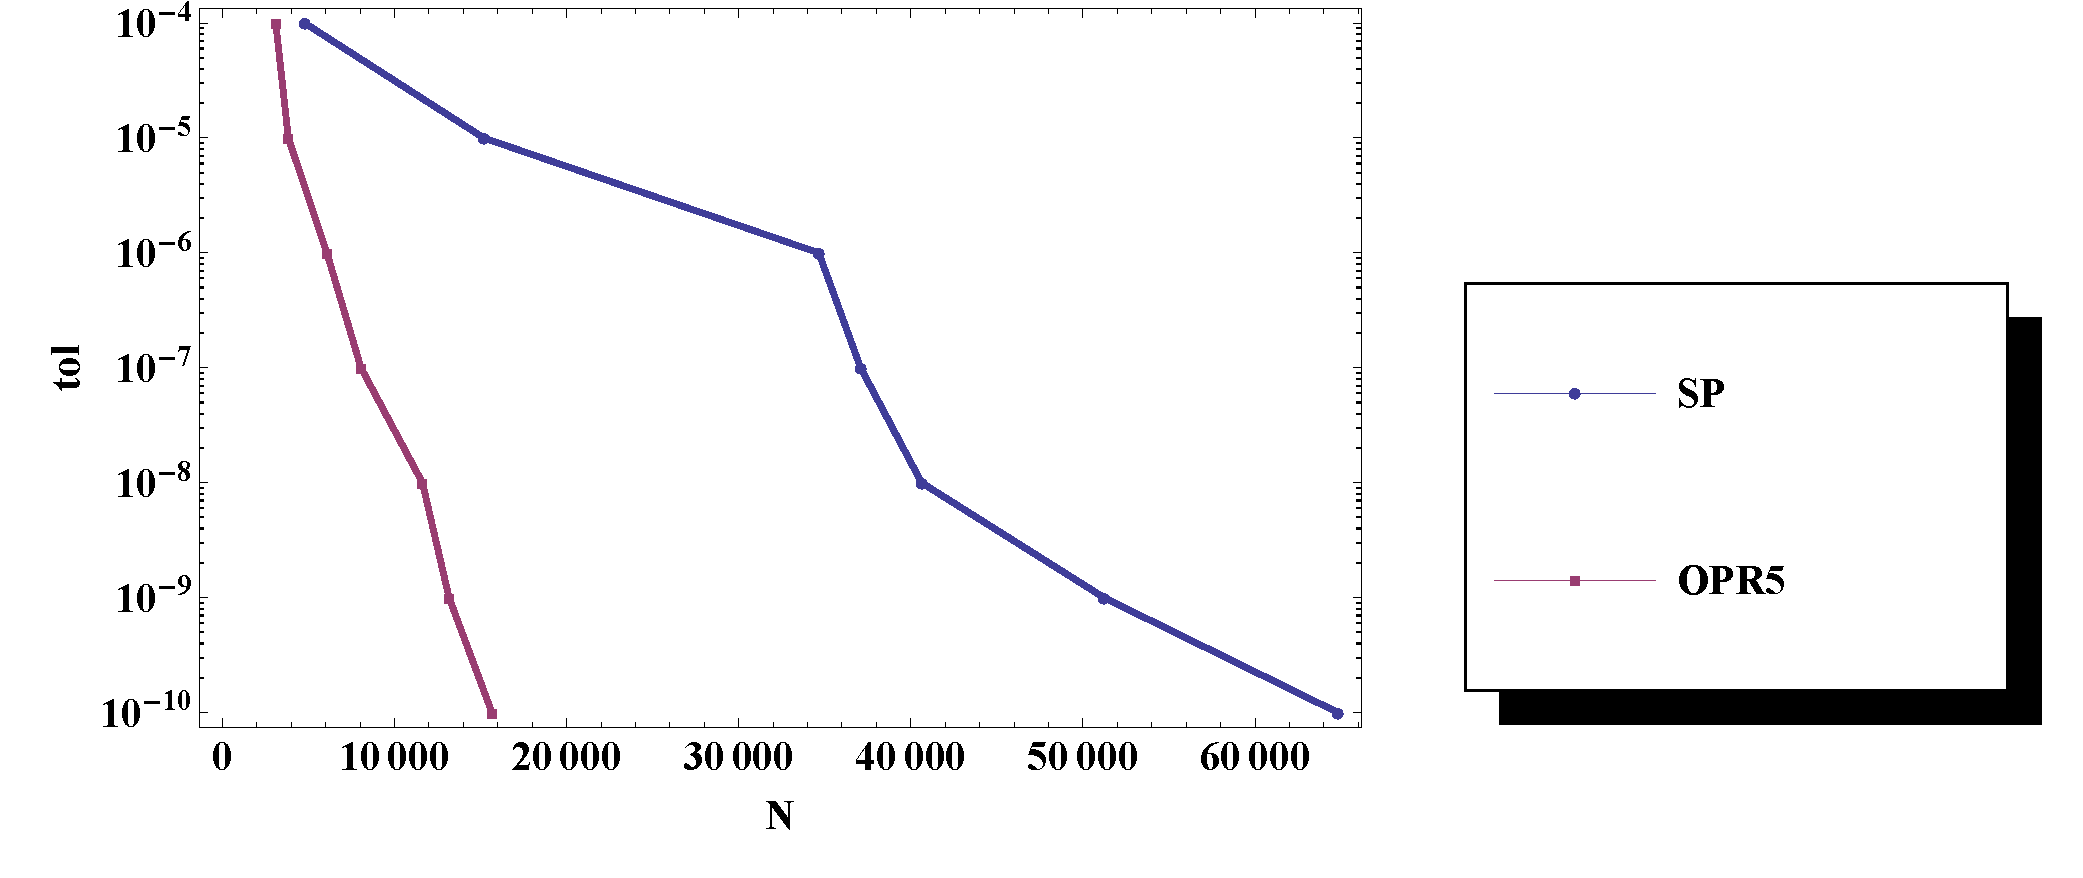
\includegraphics[height=7.3cm]{pics/num_ex_1_1.pdf}
	\caption{\small Количество итераций процесса установления SP и процесса с подавлением на каждой 5-ой итерации OPR5 при заданной точности решения}
	\label{SP_OPR5}
	\end{center}
	\end{figure}

На графике \ref{SP_OPR5} хорошо видно, что применение подавления ошибки даёт ощутимое ускорение сходимости процесса установления. При заданной точности решения $10^{-10}$ итерационный процесс без подавления практически в 4 раза медленнее сходится по сравнению с процессом с подавлением.

Попробуем происследовать, как различная частота подавления ошибки влияет на скорость сходимости. Как показал численный эксперимент (Рис. \ref{num_ex_1_2}), наилучшую скорость сходимости показал процесс с подавлением на каждой 7 итерации. Однако стоит заметить, что процессы с подавлением ошибки на 5, 7, 10, 15 итерациях сходятся с практически одинаковой скоростью, и только начиная с подавления на каждой 30 итерации, скорость сходимости уменьшается, что заметно на графике \ref{num_ex_1_2}.

	 \begin{figure}[H]
	\begin{center}
	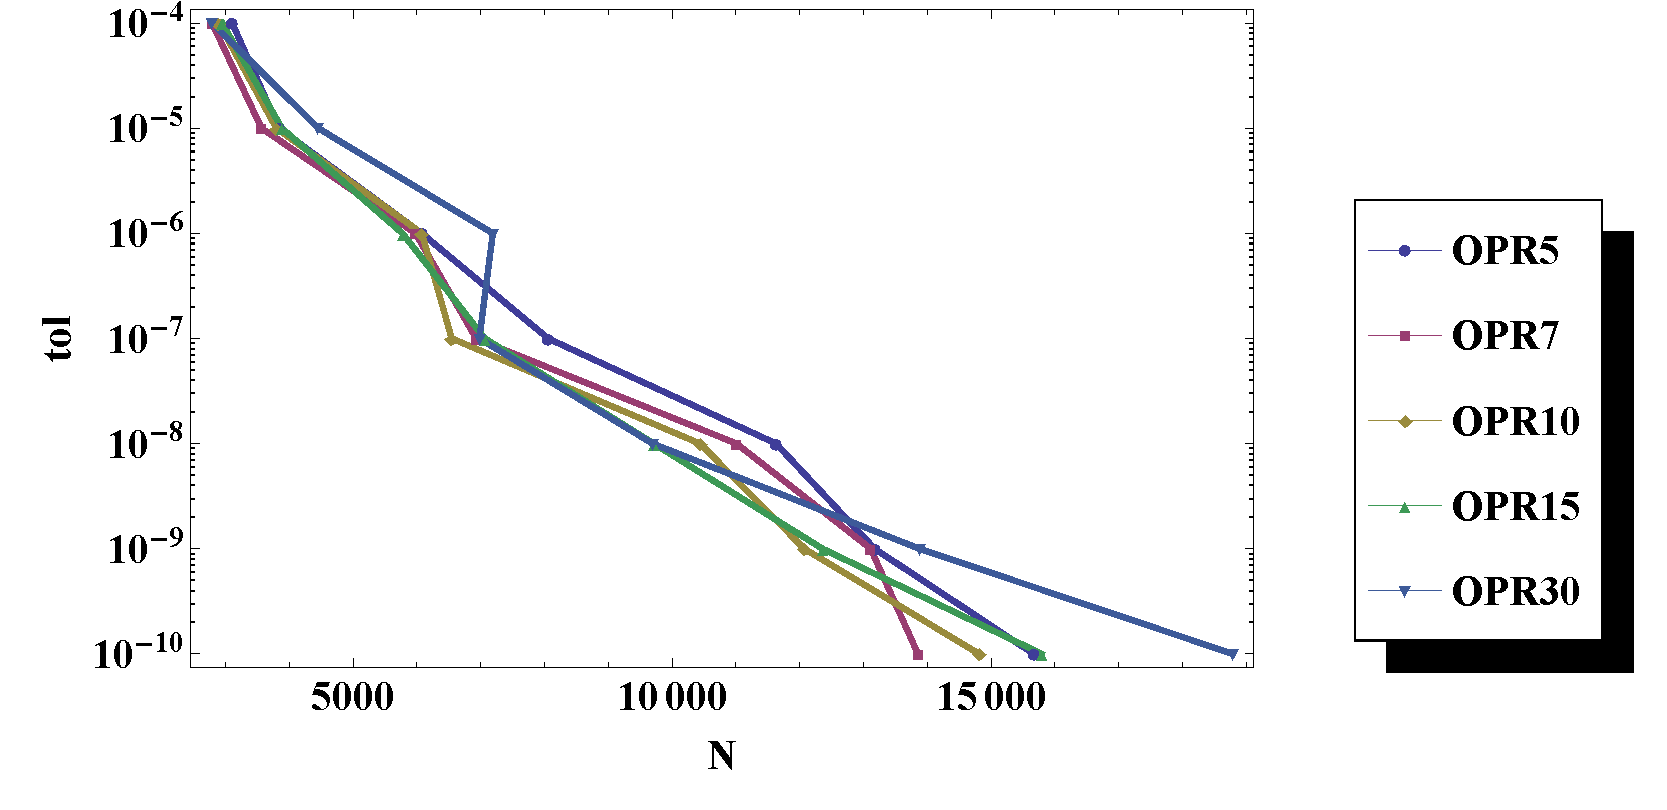
\includegraphics[height=7.3cm]{pics/num_ex_1_2.pdf}
	\caption{\small Количество итераций процессов установления OPRN с частотой подавлением на каждой N-ой итерации}
	\label{num_ex_1_2}
	\end{center}
	\end{figure}

Рассмотрим изменение нормы невязки $r$ при применении подавления на различных итерациях. В данном численном эксперименте используем описанную в главе~\ref{ss:teploprov} линейную задачу теплопроводности. Шаг по времени возьмем $\tau=0.05$, размерность задачи -- $N=20$, требуемая точность решения -- $10^{-8}$. 

	 \begin{figure}[H]
	\begin{center}
	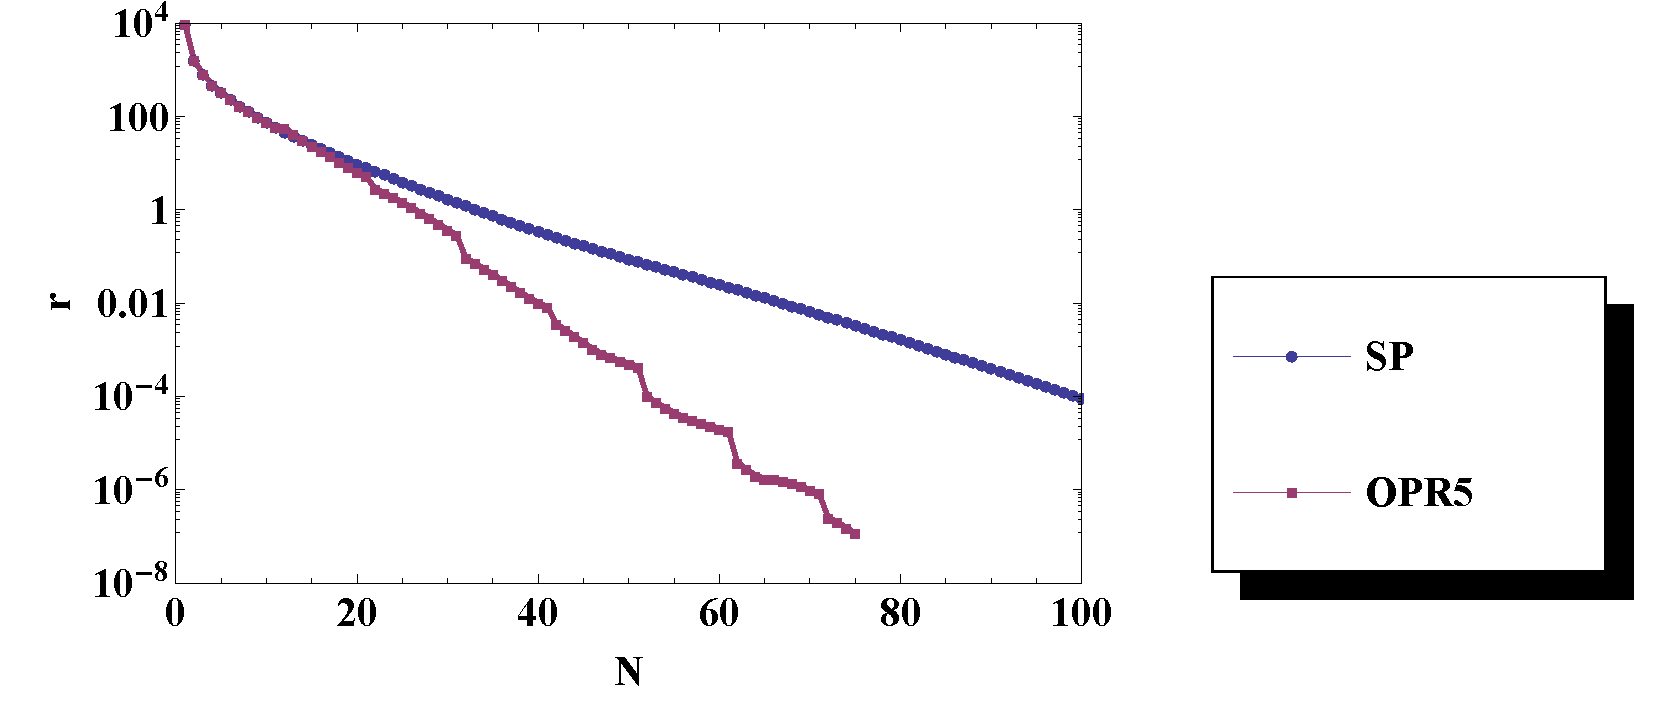
\includegraphics[height=7.3cm]{pics/num_ex_1_1_1.pdf}
	\caption{\small Норма невязки для обычного процесса установления и процесса с подавлением на каждой 5-ой итерации}
	\label{num_ex_1_3}
	\end{center}
	\end{figure}

	 \begin{figure}[H]
	\begin{center}
	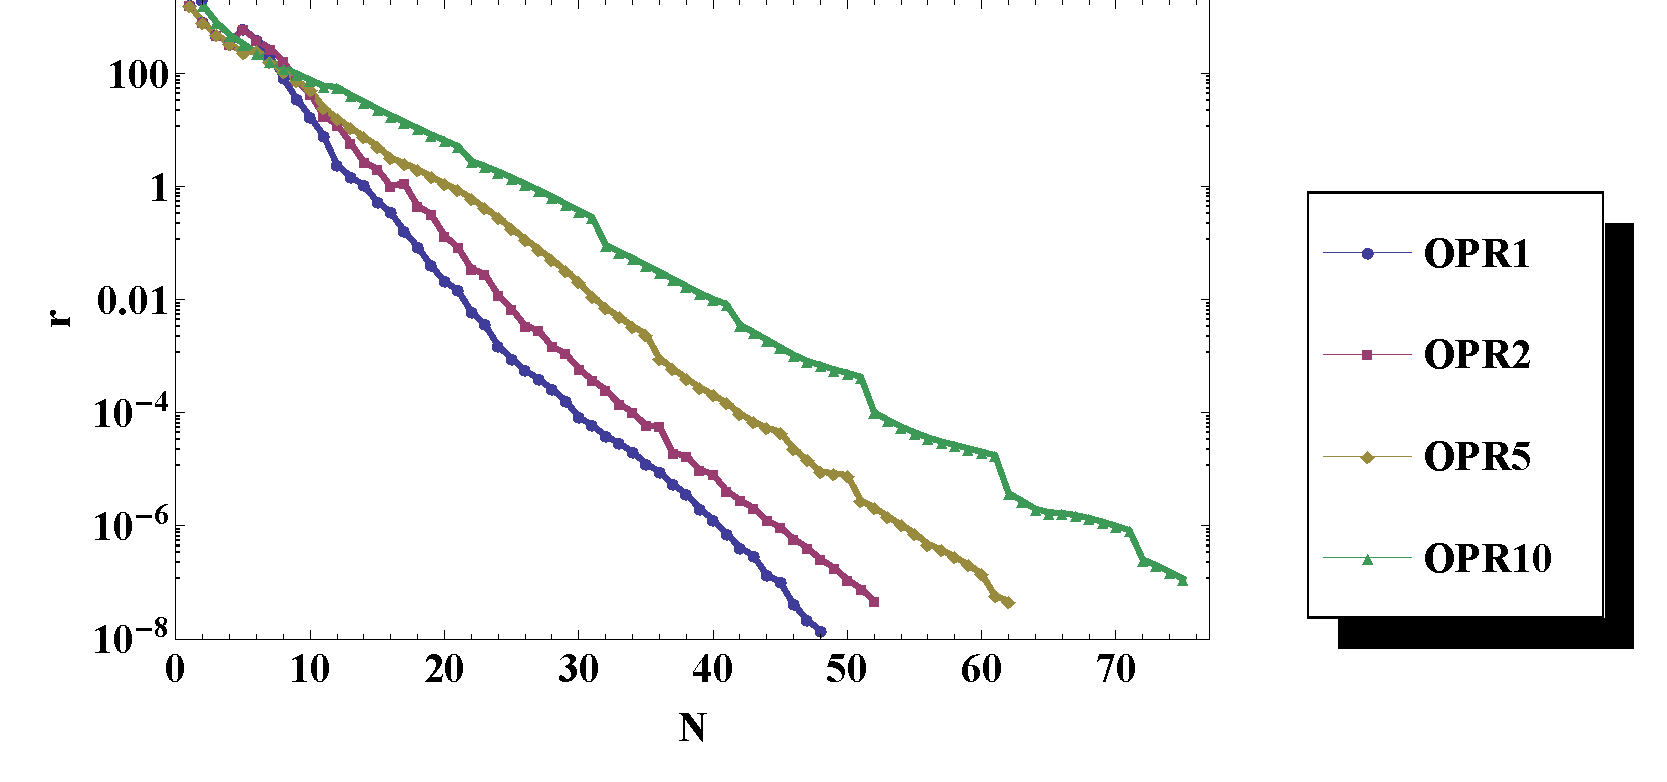
\includegraphics[height=7.3cm]{pics/num_ex_1_1_2.pdf}
	\caption{\small Норма невязки для  процессов с подавлением на каждой $N$-ой итерации}
	\label{num_ex_1_4}
	\end{center}
	\end{figure}

	
Результаты данного численного эксперимента несколько разнятся с результатами эксперимента проведенного ранее. Если в предыдущем эксперименте найлучшую скорость сходимости показал процесс с подавлением на каждой 7 итерации, то в данном эксперименте мы наблюдаем другую картину: наилучшую скорость имеет процесс с подавлением на каждой итерации. Также видно, что чем реже производить подавление, тем ниже скорость сходимости. Этот феномен требует дальнейшего изучения и исследования. 

Очевидно, что подавление компонент ошибки дает хорошее ускорение сходимости процессов установления и при этом требует небольших вычислительных затрат. 
  
  \section{Переобусловливание}
  \label{s:test_precondition}

В следующем численном эксперименте сравним скорость сходимости обычных методов установления, методов с подавлением и методов с переобусловливанием. В качестве тестовой задачи возьмем уже ранее используемую линейную задачу - одномерную задачу теплопроводности.

Однако, чтобы адекватно оценить скорость сходимости методов, недостаточно только сравнивать количества итераций процесса установления, так как операция переобусловливания в контексте применения к рассматриваемым методам является достаточно трудоемкой задачей. Поэтому также проследим за изменением количества операций перемножения матрицы на вектор и времени поиска решения для обычного и ускоренных методов установления при различной размерности тестовой задачи.

Точность искомого решения зададим $10^{-8}$. Подавление компонент ошибки будем производить на каждой итерации. В качестве переобусловливателя возьмем матрицу $J\otimes I_s$.

	 \begin{figure}[H]
	\begin{center}
	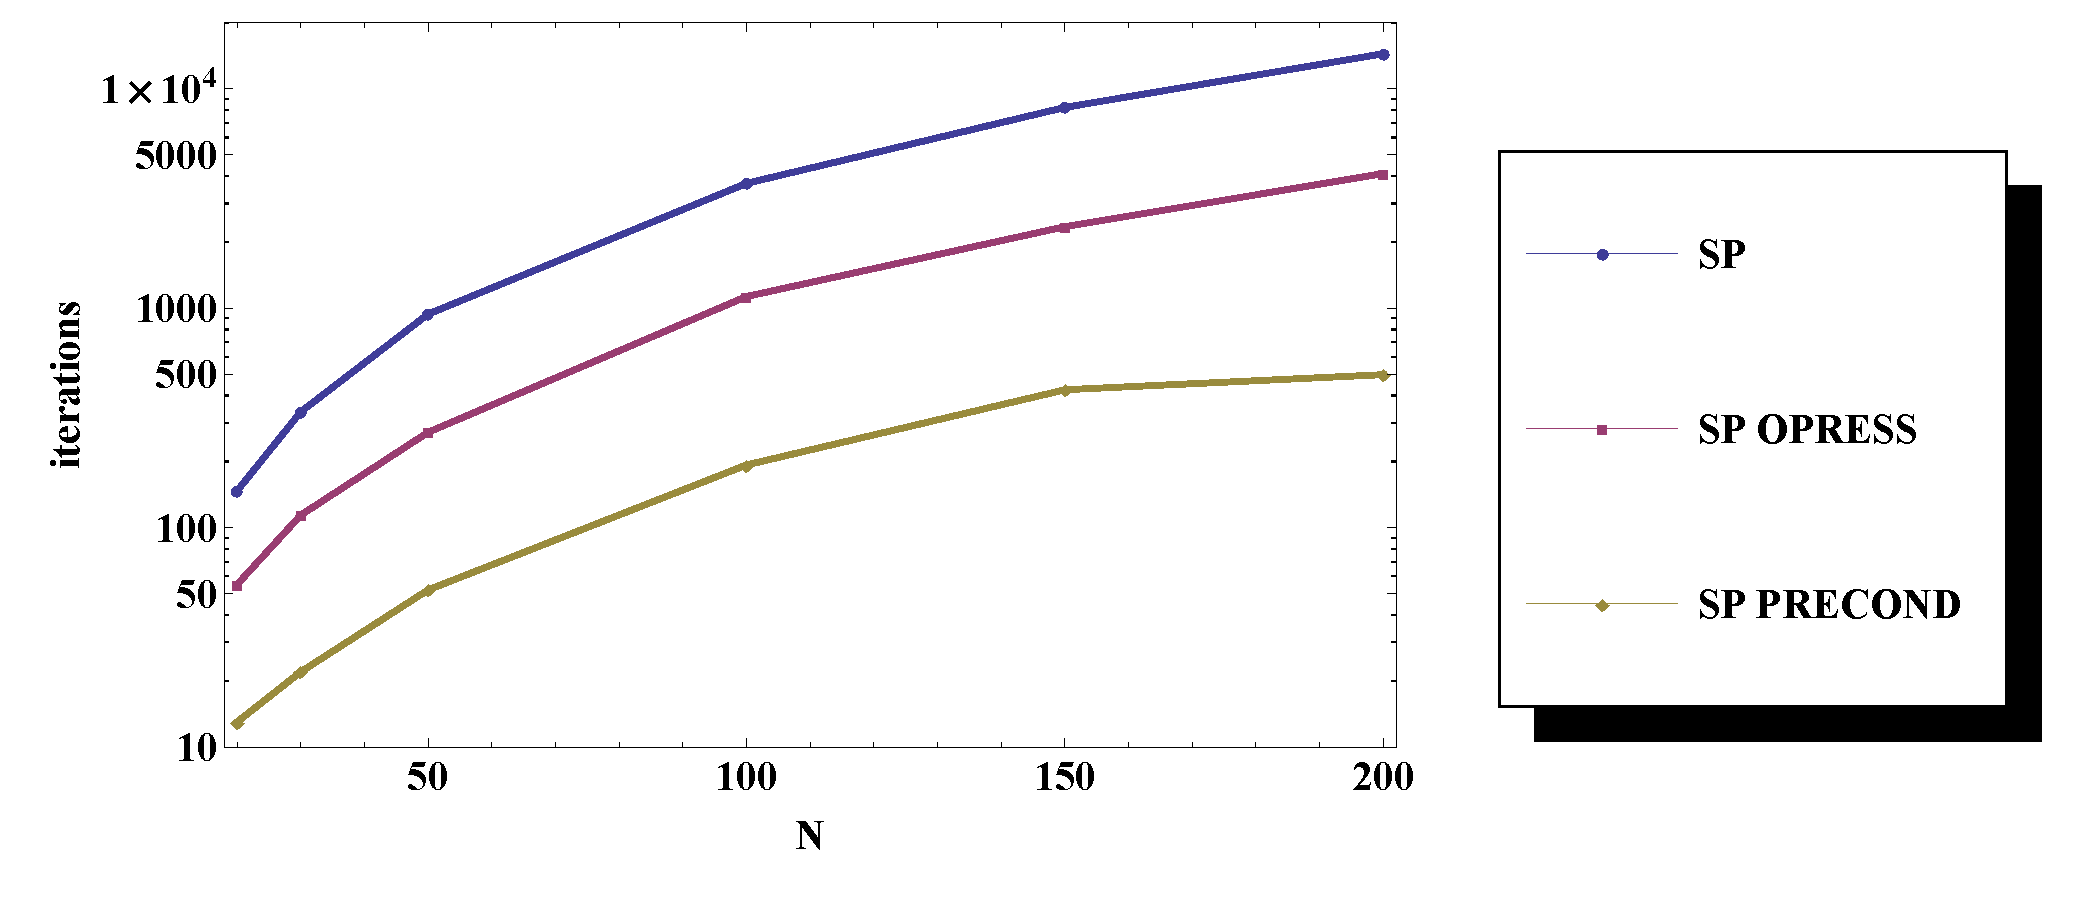
\includegraphics[height=7.3cm]{pics/num_ex_2_2_1.pdf}
	\caption{\small Количество итераций процесса установления SP, процесса с подавлением OPRESS и процесса с переобусловливанием PRECOND}
	\label{num_ex_2_2_1}
	\end{center}
	\end{figure}


	\begin{figure}[H]
	\begin{center}
	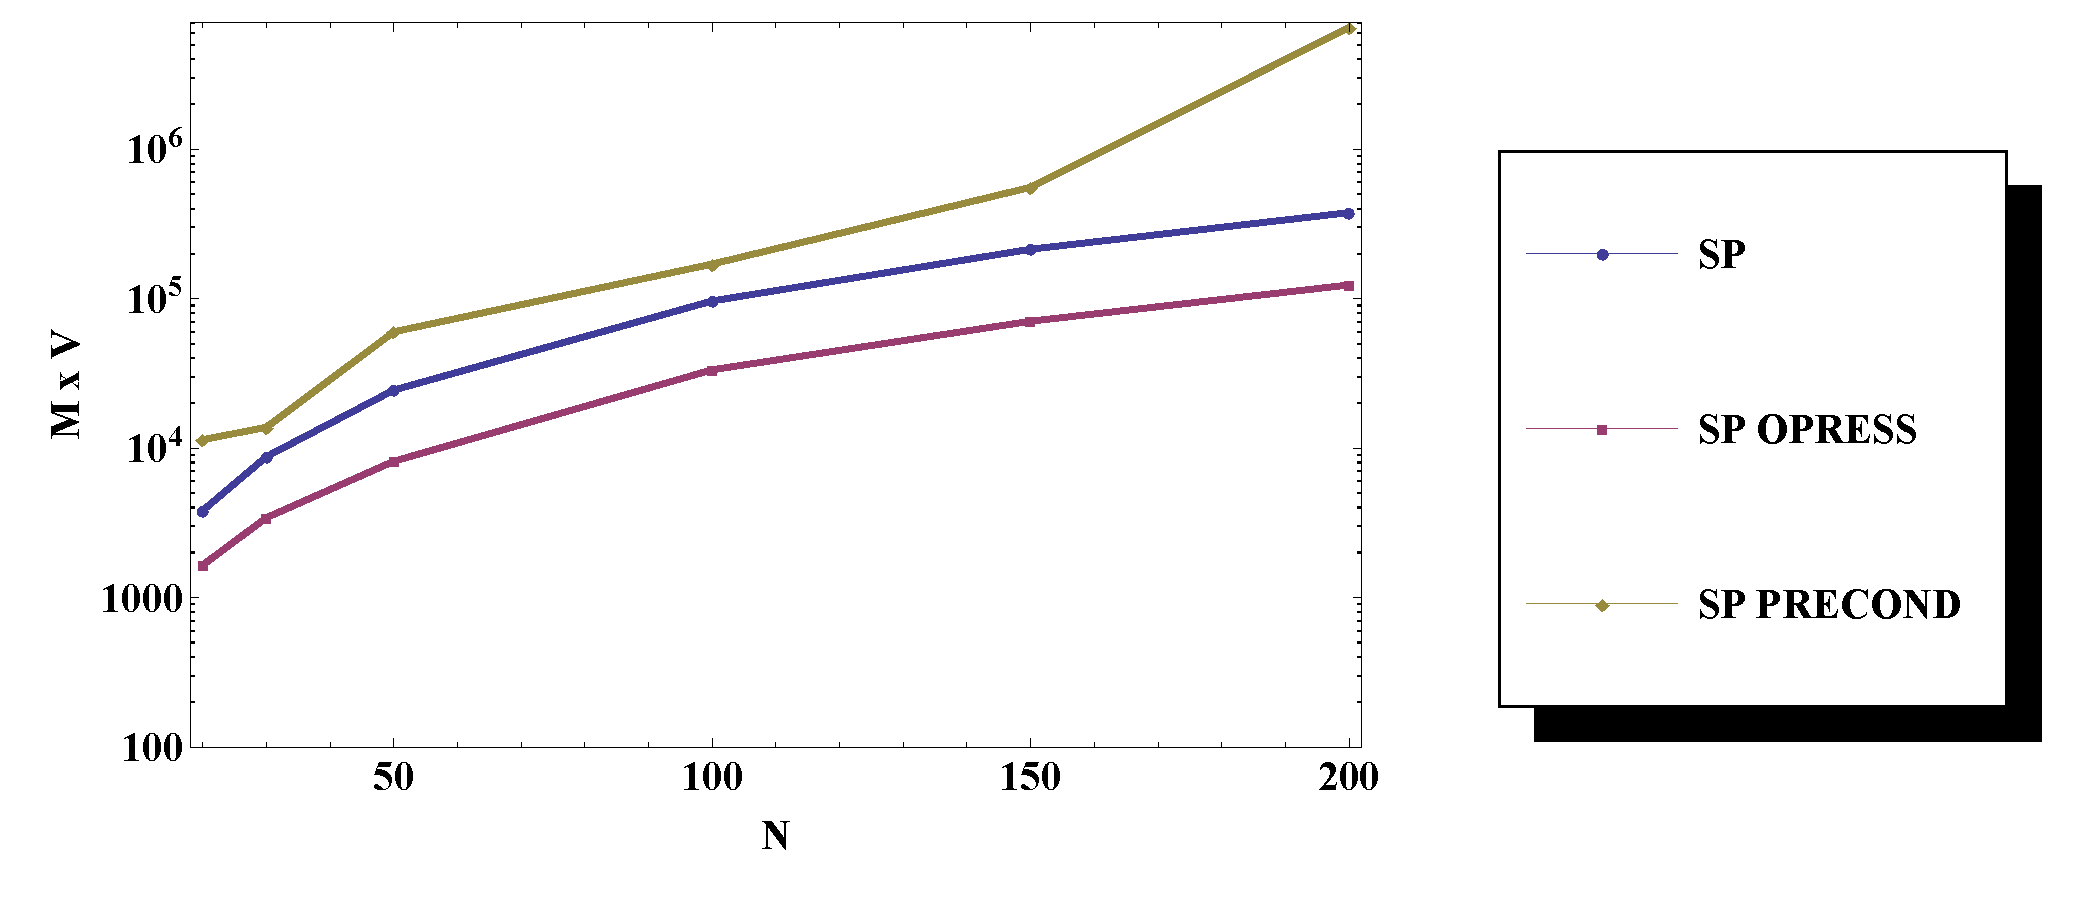
\includegraphics[height=7.3cm]{pics/num_ex_2_2_2.pdf}
	\caption{\small Количество перемножений матрицы на вектор процесса установления SP, процесса с подавлением OPRESS и процесса с переобусловливанием PRECOND}
	\label{num_ex_2_2_2}
	\end{center}
	\end{figure}

	\begin{figure}[H]
	\begin{center}
	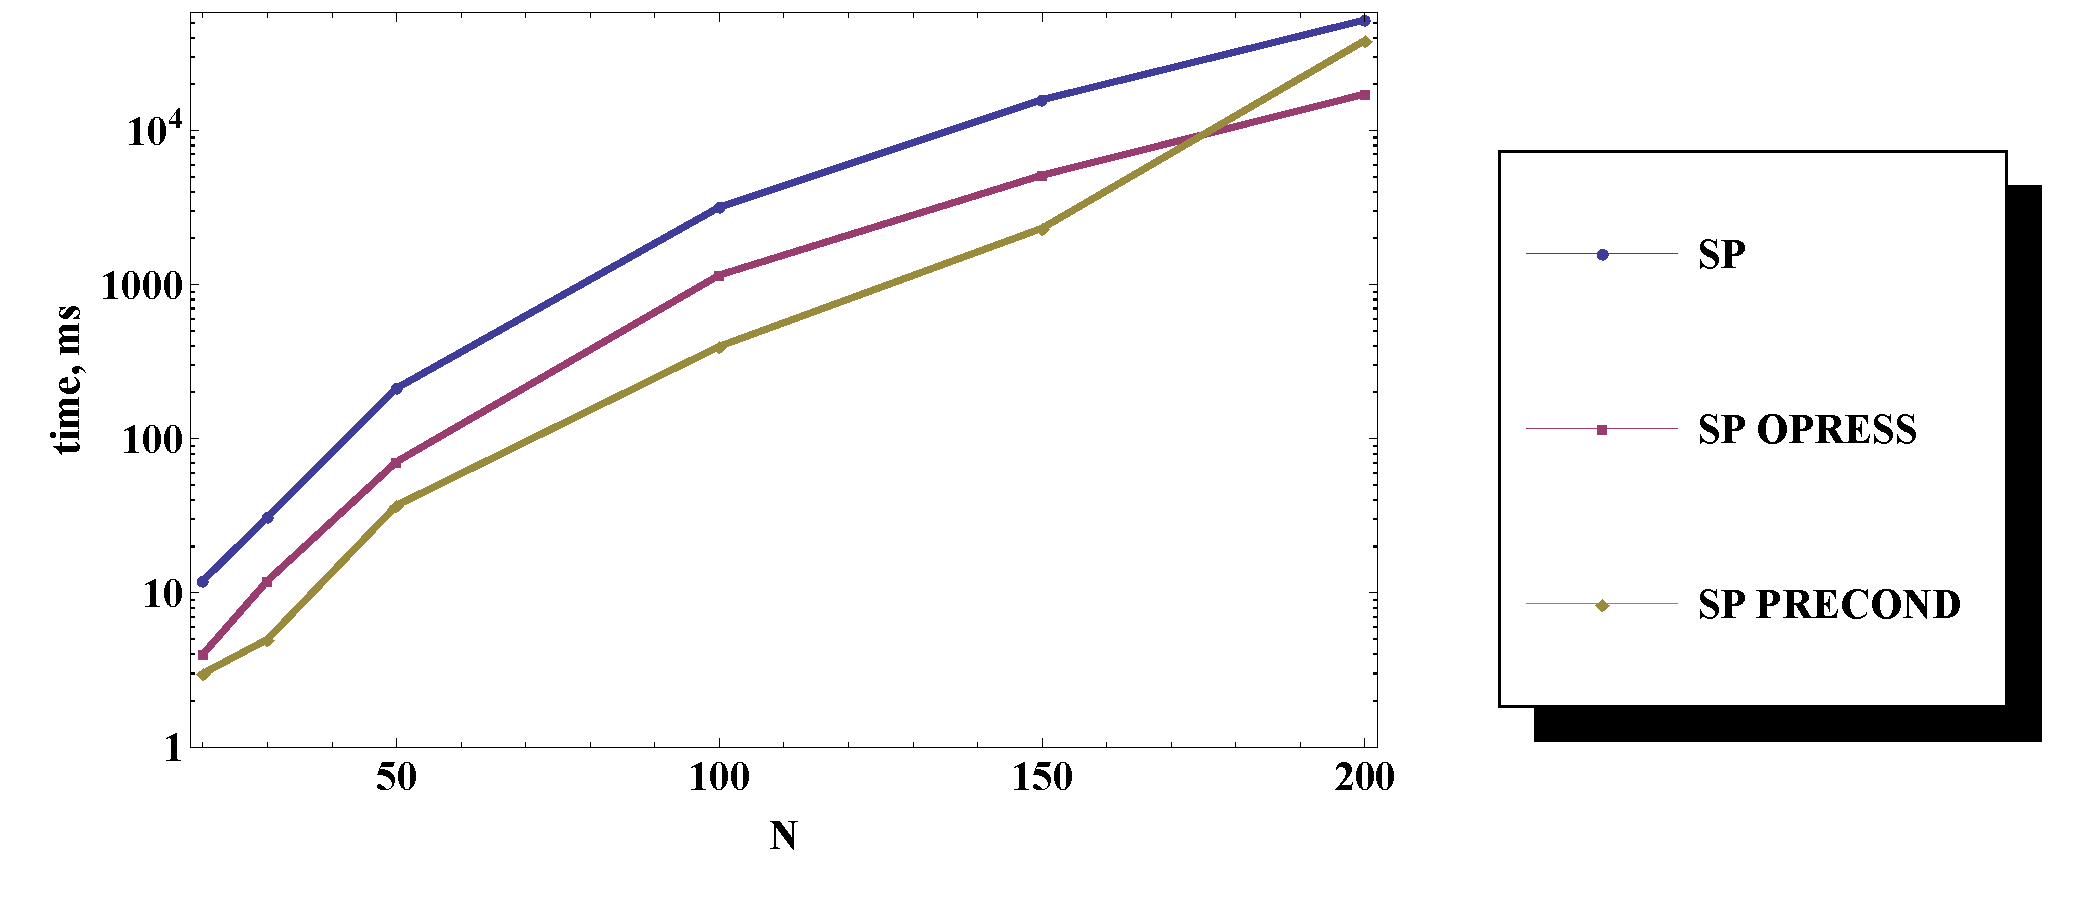
\includegraphics[height=7.3cm]{pics/num_ex_2_2_3.pdf}
	\caption{\small Время вычисления с помощью процесса установления SP, процесса с подавлением OPRESS и процесса с переобусловливанием PRECOND}
	\label{num_ex_2_2_3}
	\end{center}
	\end{figure}

Проведенный эксперимент показывает значительное ускорение сходимости процесса установления как с помощью подавления компонент ошибки, так и с помощью переобусловливания. Несмотря на значительное количество перемножений матрицы на вектор в случае способа с переобусловливанием, этот подход все же значительно превосходит обычный процесс установления во времени решения. Заметим, что подход с подавлением компонент все же предпочтительнее в случае задач большой размерности, так как в этом случае на эффективности способа с переобусловливанием сказывается трудоемкость задачи по оценке максимального собственного значения переобусловленной системы, что хорошо прослеживается на рисунке \ref{num_ex_2_2_3}.  
  
   \chapter*{Заключение}
  \addcontentsline{toc}{chapter}{Заключение}

В данной дипломной работе приведены общие принципы методов установления для решения жестких задач, рассмотрены способы ускорения сходимости итерационного процесса установления при решении систем дифференциальных уравнений. Проведен вычислительный эксперимент для линейной и нелинейной системы.

Таким образом, на основании проведенного вычислительного эксперимента на тестовой задаче HIRES и на линейной одномерной задаче теплопроводности, можно заключить, что практическая реализация способов ускорения итерационного процесса, приведенных в пунктах \ref{s:precond} и \ref{s:opress} даёт ощутимое уменьшение вычислительных затрат при использовании методов, основанных на процессе установления. Однако стоит заметить, что использование подхода, основанного на подавлении компонент ошибки, предпочтительнее в случае жестких задач больших размерностей, нежели способ с переобусловливанием.

Даже несмотря на то, что описанные в работе способы требует дальнейшего исследования и улучшения, полученые результаты вычислительного эксперимента позволяют значительно улучшить сходимость.
  
  
\newpage

\begin{thebibliography}{99}
\addcontentsline{toc}{chapter}{Литература}

\bibitem{hairer}Хайрер Э., Ваннер Г.  Решение обыкновенных дифференциальных уравнений. Жесткие и дифференциально-алгебраические задачи./ Пер. с англ. — М.: Мир, 1999. — 685 с.

\bibitem{holodov}Холодов A. С., Лобанов А. И., Евдокимов А.В. Разностные схемы для решения жестких обыкновенных дифференциальных уравнений в пространстве неопределенных коэффициентов — М.: МФТИ, 2001. — С. 45-46.

\bibitem{dekker}Деккер К., Вервер Я. Устойчивость методов Рунге—Кутты для жестких нелинейных дифференциальных уравнений/ Пер. с англ.— М.: Мир, 1988.

\bibitem{Faleichik_Bondar_Kyiv}Фалейчик Б. В., Бондарь И. В. Реализация неявных методов для жестких задач методом установления// Theoretical and Applied Aspects of Cybernetics. Proceedings of the International Scientific Conference of Students and Young Scientists -- Kyiv: Bukrek, 2011. С. 297-299.

\bibitem{Bondar_Faleichik_Parall}Bondar I. V., Faleichik B. V. Iterated Runge-Kutta Methods with Parallelization Capability for Stiff Problems // Theoretical and Applied Aspects of Cybernetics. Proceedings of the 3rd International Scientific Conference of Students and Young Scientists -- Kyiv: Bukrek, 2013. P. 336 

\bibitem{Faleichik_article}Faleichik B. V. Explicit Implementation of Collocation Methods for Stiff Systems with Complex Spectrum // Journal of Numerical Analysis, Industrial and Applied Mathematics. Vol. 5

\bibitem{Faleichik_bondar_amade}Фалейчик Б. В., Бондарь И. В. Реализация неявных методов Рунге-Кутты с использованием принципа установления //Аналитические методы анализа и дифференциальных уравнений: Тез. докл. междунар. конф. 12-17 сент. 2011г, Минск, Беларусь. С. 146-147

\bibitem{Faleichik_amade}Фалейчик Б. В. Реализация неявных методов для жестких задач с использованием обобщенных итераций Пикара // Тр. 6-й международной конференции «Аналитические методы анализа и дифференциальных уравнений»: в двух томах – Т.1 Математический анализ. — Минск: Институт математики НАН Беларуси, 2012. С. 131–135.

\bibitem{gomel}Фалейчик Б. В., Бондарь И. В. Реализация неявных методов Рунге-Кутты для больших жестких систем//Новые математические методы и компьютерные технологии в проектировании, производстве и научных исследованиях: XV Республиканская научная конференция студентов и аспирантов ``Новые математические методы и компьютерные технологии в проектировании, производстве и научных исследованиях'', 26-28 марта 2012 г.:[материалы]: в 2 ч. Ч.1/редкол. : Демиденко О.М. -- Гомель: ГГУ им. Ф. Скорины, 2012. С. 175-176

\bibitem{konf_may}Бондарь И. В. Итерационные процессы установления для жестких линейных задач //Тр. 69-й ежегодной научной конференции студентов и аспирантов БГУ: допущено в печать.

\bibitem{Bondar}Бондарь И. В. Итерационные процессы установления для жестких задач //Республиканский конкурс научных работ студентов высших учебных заведений: допущено в печать.

\bibitem{Faleichik_Vych_alg}Фалейчик Б. В. Вычислительные алгоритмы решения жестких задач на основе процессов установления // Труды института математики НАН Беларуси. -- 2004. -- Т. 12, № 1. -- С. 45-48.

\bibitem{benzi}Benzi M. Preconditioning Techniques for Large Linear Systems: A Survey // Journal of Computational Physics. Vol.182, 2002. P. 418-477.

\bibitem{chen}Chen K. Matrix Preconditioning Techniques and Applications // Cambridge University Press, 2005, P. 195-197.

\bibitem{fadeev}Фадеев, Д.К., Фадеева, В.Н. Вычислительные методы линейной алгебры // М:Физматгиз, 1963. -- С. 570-572.

\bibitem{wiki-precond} Интернет адрес: https://ru.wikipedia.org/wiki/Предобуславливание
\end{thebibliography}


  \appendix
\end{document}
